\documentclass{article}
\usepackage[utf8]{inputenc}


\title{The Perfect Study Buddy: AI Generated Study Music}
\author{Ellen Moore, Tyler Chang, Lena Fleischer}
\date{18 September 2022}

\usepackage{graphicx}
\usepackage[margin=1in]{geometry}

\graphicspath{ {./images/} }
\begin{document}

\maketitle

\section{Abstract}
We aim to generate study music based on classical piano pieces using natural language processing (NLP) techniques. With there being many robust techniques in NLP, we investigate if we can apply these methodologies to music generation by treating music as a language. By utilizing a dataset of over 100 classical piano pieces in the MIDI file format, the generation process is broken down into three major components: a right hand melody track, a left hand harmony accompaniment track, and rhythmic variation. By applying the n-gram generation technique for the melody and the Hidden Markov Model for the harmony and rhythm, the audio result presents a clear composition of a melodic line accompanied by harmonic chords with a variety of rhythms. However, it is far from a composition by an actual human. Though the NLP techniques that were implemented have been proven to provide good results, the dataset, particularly due to the MIDI library in use, provided limitations in obtaining tempo and note durations which led to difficulty in data processing for the models. Moving forward, further research in other techniques in NLP such as neural networks and autoencoders may serve to provide an even better result.

\section{Introduction}
We are interested in exploring the language of music, particularly “study music”, a genre which we as students encounter frequently in our day-to-day academic lives. This project aims at digging into some questions: What kinds of music are most conducive to studying? How can we generate original music that is optimal for studying? Using natural language processing techniques, we create an AI to auto generate music that will be unique and conducive to studying. Using the “Classical Piano Midi Page” \cite{Mozart}, we download MIDI files to create a database to train our model. In this investigation, we take a three pronged approach by targeting three key musical components: melody, harmony, then rhythm. 

\section{Background}
From generating Beethoven symphonies to writing lyrics, AI generated music has been present since the early stages of digital technology and has been improving drastically in the recent years with the help of machine learning. Jukebox, a generative music model by OpenAI  \cite{jukebox}, is currently a leading example of music generation utilizing neural networks. Instead of generating music symbolically in the form of a piano roll, Jukebox chooses to model music directly as raw audio data in order to capture human voices, subtle timbres, dynamics, and expressivity which are all essential towards realistic generation. By utilizing neural networks and an autoencoder model to compress the data into discrete spaces, Jukebox is able to generate not only a song in a particular genre, but also in the style of a certain artist from the genre. In contrast to this audio data based approach, we became interested in representing music as a language. Here, we apply NLP concepts, taking a symbolic approach of music generation and exploring a variety of ideas of applying it with NLP techniques to music. We ended up taking some inspiration from “Representing music with Word2vec?” \cite{word2vec}, which discusses an application of word2vec techniques, applied to “slices” of music. Another article, “Generating Music Using Deep Learning” \cite{deep-learning} increased our understanding of using deep learning methods and vectors with music.

\begin{figure}[ht]
\centering
\fbox{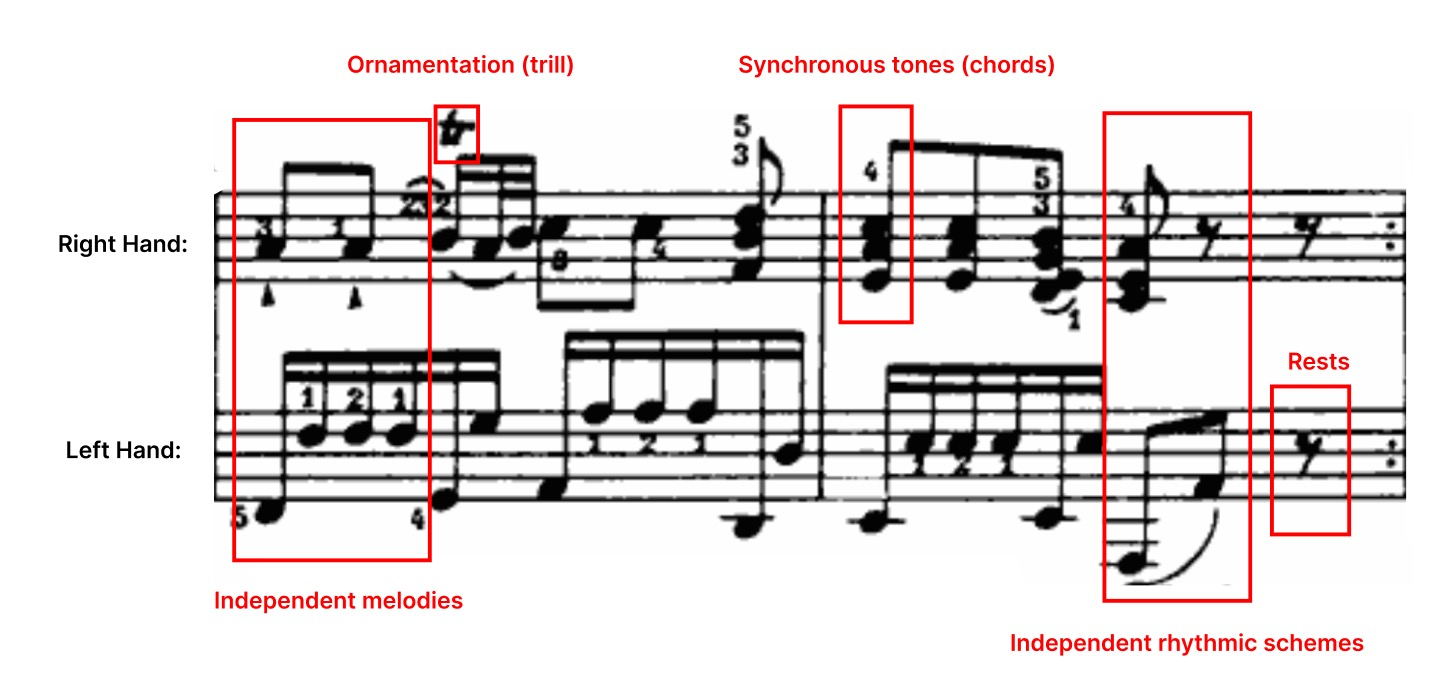
\includegraphics[width= 10cm]{musical_complexity_fig}}
\caption{Passage from Mozart's Sonata No.11, annotated to display complexity of classical music.\cite{sheetmusic}.}
\end{figure}

\par Due to numerous studies on how classical music helps and improves studying, we have decided to use a dataset of classical music to train our model in order to generate music in a similar style. By working with classical music, we have the benefit of a large corpus, but are still limited by its complexity (see figure 1). Complicating factors include: multiple instruments in a single song, compositions in various musical keys, complex rhythms, and combinations of both asynchronous notes and synchronous notes (chords.) An additional complication lies in that much of classical music is polyphonic, meaning that it contains multiple independent melodies layered on top of one another, often each with their own rhythmic scheme. We have taken a few simplifying measures in order to reduce the complexity of our task for version one. 


\section{Data}
Using the “Classical Piano MIDI Page” \cite{Mozart}, we downloaded a selection of pieces from Chopin, Debussy, Liszt, Mozart, and Tchaikovsky, yielding 104 total MIDI files for training. The MIDI file format is the technical standard communications protocol between an electronic instrument and a computer. To process these pieces, we used the Mido python library \cite{midodoc}. Garageband \cite{garageband} was used to produce audio from output MIDI files. 

\begin{figure}[ht]
\centering
\fbox{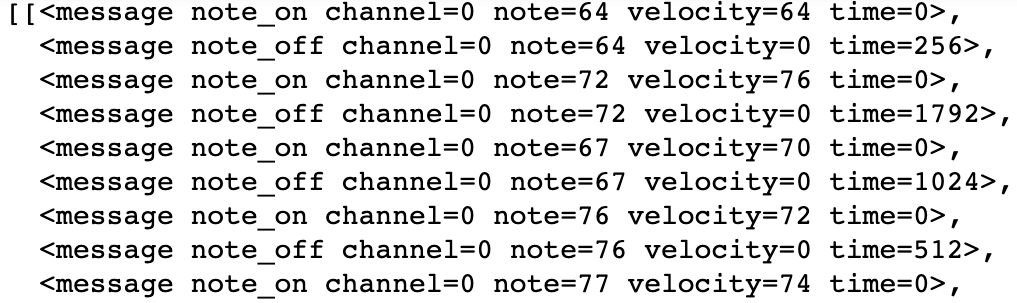
\includegraphics[height= 2.5cm]{message2}}
\fbox{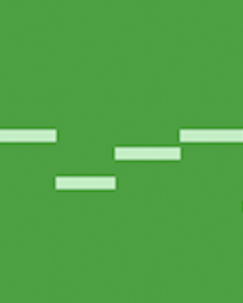
\includegraphics[height= 2.5cm]{right-garage2}}
\caption{The left image is the notes represented in messages and the right image is the notes represented in garage band.}
\end{figure}

\section{Methods}
\subsection{Melody Generation}
As our first step, we create piano melodies using an n-gram bag of words approach. Since this step focuses on melody, rhythmic variation is ignored for the time being. 
\par To focus on the melody, the right hand part is selected from a selection of classical piano scores. In classical piano music, this track conventionally contains a monotonic melody. To deal with the issue of compositions in different keys, we transpose all songs so that they have one consistent key signature. By processing the songs, we were able to create a corpus with one unified key signature, as opposed to the 12 different key signatures that the raw input data would yield. For this purpose, major and minor keys were treated the same (i.e. songs in C major are dealt with in the same way as songs in the relative minor key, A minor.) 
\par We first create a list of note value token sequences from right hand data to create an ngram probability dictionary. To generate a new token, note values are sequentially chosen based on the n-1 previous tokens. The resulting output song consists of a sequence of notes, each sustaining for one beat, in the key of C major.


\subsection{Harmony Generation}
In our first step, we created a melody for the right hand piano track. In order to generate the left hand (harmony) sequence, we wanted to make sure that a generated left hand note not only accompanied the right hand note at that time but also makes sense in the entire left hand note sequence.  To achieve this, a hidden Markov model was implemented to map our right hand “observable” states to left hand “hidden states.”  By using the left hand notes in our training data as our target hidden state, we “slice” each right hand note and pair it with its corresponding left hand note. From our lists of notes and times, we compare the left hand against the right hand to select notes that are playing at the same time. This informs emission probabilities from left hand to right hand states. We then use the Viterbi algorithm to create possible melodies. 

\begin{figure}[ht]
\centering
\fbox{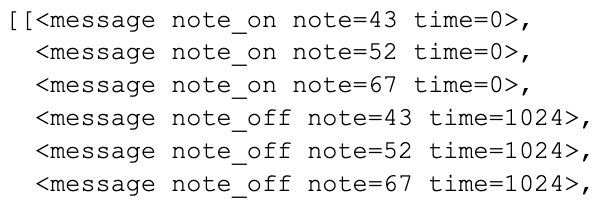
\includegraphics[width= 5cm]{chord}}
\fbox{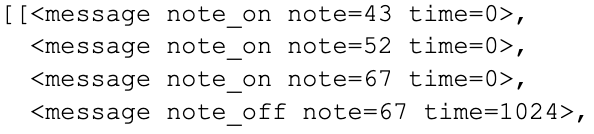
\includegraphics[width= 5cm]{images/otherChord.png}}
\caption{The right and left images below represent the same chord. We had trouble reading in chords because ad the right image shows, sometimes the notes don't have a note\_off.}
\end{figure}

\par A roadblock was presented when we discovered that MidiFiles, Mido’s representation of MIDI objects, do not keep track of an absolute time. Each note is associated with its duration, represented in “messages”, where a “note\_on” (notename) message indicates the note’s name, and a “note\_off” (duration) message indicates the duration of that note. This gets complicated when chords are involved, in which case they are represented by a sequence of notename messages, followed by duration messages, in an arbitrary order. In some cases, no “note\_off” duration is specified.(See figure 1.) These factors made for a significant challenge in figuring out emission probabilities. 
\par In an attempt to deal with this problem, we first iterate through the messages, reading in only notename messages directly followed by duration messages, or in the case of chords, reading in only the first listed note and its corresponding duration message. This results in only reading in one note per chord. created a two-pronged method, in which we create a list of notes for each hand, associated with a list of times for that hand. In testing this, however, we are still finding a slight misalignment. With further investigation, we found general inconsistencies with the time attribute in our pipeline from MIDI generation to Garageband audio. It appears that, while mido \cite{midodoc} defines the time attribute as keeping track of a “delta time”, these times do not directly impact the duration of notes in audio clip. 
\par We were able to generate melodies with correlating harmony, though a qualitative review indicates that the harmony note selection creates a more dissonant song than we would like. This is almost certainly due to the aforementioned misalignment in the emission probability creation. 


\subsection{Adding Rhythmic Variation}
 In the melody and harmony AI versions, we have one rhythm throughout the duration of the song (each note gets one beat.) Now, we explore using a hidden Markov model to assign rhythmic value to notes, similar to the way we generated a left hand accompaniment. Since each note has an associated time attribute attached with it which represents the duration, we created an adjacent list of all the durations for each note in a song as our hidden state. From there, it was a matter of generating another set of transition and emission probabilities for left and right hand durations. After running it through the Viterbi algorithm, we now not only had a set of right and left hand notes, but also a list of durations for each note. As a result, we were able to get audible rhythmic variety in our tracks which increased the originality of the generated song, while making it more interesting to listen to. However, due to the inconsistent nature of the time (duration) attribute from the Mido library, it was difficult to conclude if our generated durations were being played as intended.
 
\section{Results}
In the end, we were able to generate new study music but we wanted to make sure the generated music was unique. We used PyRouge’s rouge\_metric  \cite{rouge}.  From this, we were able to generate the recall, precision, and f1 for both the right and left hands. By comparing our output song against all input songs, we were able to measure the originality of our output music. The maximum results are shown in Figure 4. The right hand is consistently more unique than the left. 

\begin{figure}[ht]
\centering
\fbox{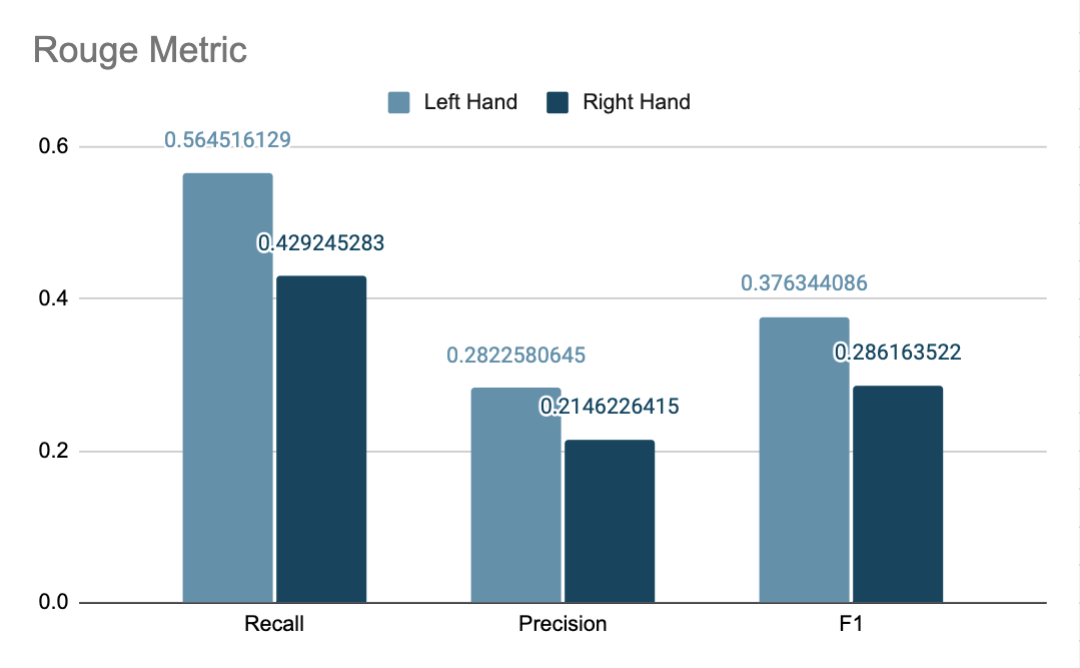
\includegraphics[width= 10cm]{rouge}}
\caption{We used ROUGE metric to compute the recall, precision, and f1 for the right hand and the left hand. This chart shows the max values of each.}
\end{figure}

\section{Conclusions}
In this work we proposed a method for study music generation using an ngram bag of words model for melody generation, coupled with hidden Markov models to create harmony and rhythmic variation. Due to some setbacks presented by our processed input data from the Mido library (difficulty interpreting messages and inconsistency of Mido’s time attribute,) we were limited in the quality of songs we could produce. Going forward, we would like to try out different MIDI processing libraries, or even create our own flexible MIDI processing software. Eliminating processing issues would fix problems with note misalignment and messages, and therefore rhythm. We look forward to taking on this data processing challenge and trying out different NLP techniques, such as autoencoder networks, in future work. 






\pagebreak
\begin{thebibliography}{9}
\bibitem{sheetmusic}
Admin, and Admin. “Piano Sonata No.11 in a Major, K.331 (Wolfgang Amadeus Mozart).” SHEET MUSIC CATALOG OF CLASSICAL MUSIC, 2 May 2022, https://musopus.net/piano-sonata-no-11-in-a-major-k-331-wolfgang-amadeus-mozart/\#google\_vignette.

\bibitem{garageband}
“GarageBand for Mac.” Apple, https://www.apple.com/mac/garageband/.

\bibitem{word2vec}
Herremans, Dorien. “Representing Music with word2vec?” Medium, Towards Data Science, 7 May 2019, https://towardsdatascience.com/representing-music-with-word2vec-c3c503176d52.

\bibitem{Mozart}
Krueger, Bernd. “Mozart.” Classical Piano Midi Page - Mozart, http://www.piano-midi.de/mozart.htm.

\bibitem{midodoc}
“MIDI Objects for Python¶.” Mido, https://mido.readthedocs.io/en/latest/. 

\bibitem{jukebox}
OpenAI. “Jukebox.” OpenAI, OpenAI, 21 June 2021, https://openai.com/blog/jukebox/. 

\bibitem{rouge}
“Rouge-Metric.” PyPI, https://pypi.org/project/rouge-metric/. 

\bibitem{deep-learning}
Tham, Isaac. “Generating Music Using Deep Learning.” Medium, Towards Data Science, 30 Aug. 2021, https://towardsdatascience.com/generating-music-using-deep-learning-cb5843a9d55e. 
]
\end{thebibliography}

\end{document}
